\documentclass{article}
\usepackage{tikz,amsmath}
\title{CSC 320 Assignment 1}
\author{Oliver Tonnesen\\V00885732}
\date{January 29, 2019}
\begin{document}
\maketitle
\renewcommand{\thesubsection}{\thesection.\alph{subsection}}
\section{} % Section 1
\subsection{} % Section 1.a
\begin{minipage}{\textwidth}
\begin{center}
	\begin{tikzpicture}[scale=0.2]
		\tikzstyle{every node}+=[inner sep=0pt]
		\draw [black] (13.2,-30.1) circle (3);
		\draw (13.2,-30.1) node {$q_1$};
		\draw [black] (38.1,-30.1) circle (3);
		\draw (38.1,-30.1) node {$q_2$};
		\draw [black] (65.2,-30.1) circle (3);
		\draw (65.2,-30.1) node {$q_3$};
		\draw [black] (65.2,-30.1) circle (2.4);
		\draw [black] (38.1,-16.7) circle (3);
		\draw (38.1,-16.7) node {$q_4$};
		\draw [black] (6.8,-30.1) -- (10.2,-30.1);
		\fill [black] (10.2,-30.1) -- (9.4,-29.6) -- (9.4,-30.6);
		\draw [black] (16.2,-30.1) -- (35.1,-30.1);
		\fill [black] (35.1,-30.1) -- (34.3,-29.6) -- (34.3,-30.6);
		\draw (25.65,-29.6) node [above] {$0,1$};
		\draw [black] (41.1,-30.1) -- (62.2,-30.1);
		\fill [black] (62.2,-30.1) -- (61.4,-29.6) -- (61.4,-30.6);
		\draw (51.65,-29.6) node [above] {$1$};
		\draw [black] (38.1,-27.1) -- (38.1,-19.7);
		\fill [black] (38.1,-19.7) -- (37.6,-20.5) -- (38.6,-20.5);
		\draw (38.6,-23.4) node [right] {$0$};
		\draw [black] (65.275,-27.113) arc (206.29243:-81.70757:2.25);
		\draw (70.08,-23.62) node [above] {$0,1$};
		\fill [black] (67.62,-28.34) -- (68.56,-28.44) -- (68.11,-27.54);
		\draw [black] (37.57,-13.759) arc (217.94629:-70.05371:2.25);
		\draw (41.39,-9.62) node [above] {$0,1$};
		\fill [black] (40.11,-14.49) -- (41.05,-14.39) -- (40.44,-13.6);
	\end{tikzpicture}
\end{center}

\end{minipage}
\subsection{} % Section 1.b
\begin{minipage}{\textwidth}
\begin{center}
	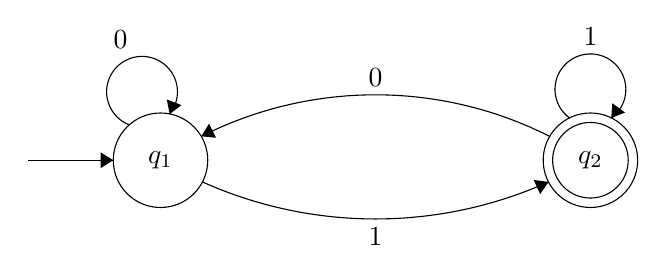
\begin{tikzpicture}[scale=0.2]
		\tikzstyle{every node}+=[inner sep=0pt]
		\draw [black] (24.2,-31) circle (3);
		\draw (24.2,-31) node {$q_1$};
		\draw [black] (51.5,-31) circle (3);
		\draw (51.5,-31) node {$q_2$};
		\draw [black] (51.5,-31) circle (2.4);
		\draw [black] (15.8,-31) -- (21.2,-31);
		\fill [black] (21.2,-31) -- (20.4,-30.5) -- (20.4,-31.5);
		\draw [black] (48.837,-32.378) arc (-65.8424:-114.1576:26.847);
		\fill [black] (48.84,-32.38) -- (47.9,-32.25) -- (48.31,-33.16);
		\draw (37.85,-35.23) node [below] {$1$};
		\draw [black] (26.787,-29.485) arc (116.84792:63.15208:24.496);
		\fill [black] (26.79,-29.48) -- (27.73,-29.57) -- (27.28,-28.68);
		\draw (37.85,-26.34) node [above] {$0$};
		\draw [black] (22.225,-28.757) arc (249.10435:-38.89565:2.25);
		\draw (21.67,-23.92) node [above] {$0$};
		\fill [black] (24.78,-28.07) -- (25.53,-27.5) -- (24.6,-27.14);
		\draw [black] (50.177,-28.32) arc (234:-54:2.25);
		\draw (51.5,-23.75) node [above] {$1$};
		\fill [black] (52.82,-28.32) -- (53.7,-27.97) -- (52.89,-27.38);
	\end{tikzpicture}
\end{center}

\end{minipage}
\subsection{} % Section 1.c
\begin{minipage}{\textwidth}
\begin{center}
	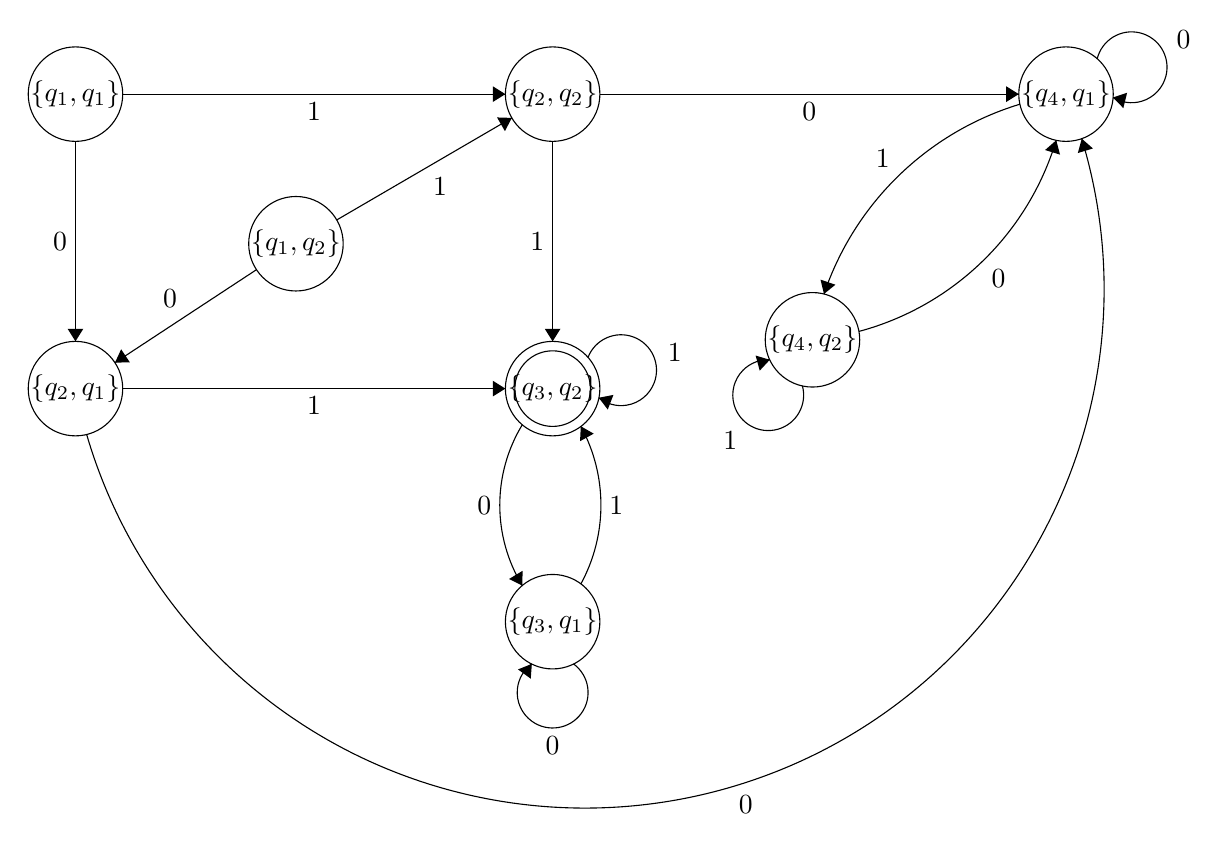
\begin{tikzpicture}[scale=0.2]
		\tikzstyle{every node}+=[inner sep=0pt]
		\draw [black] (8.4,-6.4) circle (3);
		\draw (8.4,-6.4) node {$\{q_1,q_1\}$};
		\draw [black] (38.7,-6.4) circle (3);
		\draw (38.7,-6.4) node {$\{q_2,q_2\}$};
		\draw [black] (71.3,-6.4) circle (3);
		\draw (71.3,-6.4) node {$\{q_4,q_1\}$};
		\draw [black] (8.4,-25.1) circle (3);
		\draw (8.4,-25.1) node {$\{q_2,q_1\}$};
		\draw [black] (38.7,-25.1) circle (3);
		\draw (38.7,-25.1) node {$\{q_3,q_2\}$};
		\draw [black] (38.7,-25.1) circle (2.4);
		\draw [black] (55.2,-22) circle (3);
		\draw (55.2,-22) node {$\{q_4,q_2\}$};
		\draw [black] (38.7,-39.9) circle (3);
		\draw (38.7,-39.9) node {$\{q_3,q_1\}$};
		\draw [black] (22.4,-15.9) circle (3);
		\draw (22.4,-15.9) node {$\{q_1,q_2\}$};
		\draw [black] (11.4,-6.4) -- (35.7,-6.4);
		\fill [black] (35.7,-6.4) -- (34.9,-5.9) -- (34.9,-6.9);
		\draw (23.55,-6.9) node [below] {$1$};
		\draw [black] (41.7,-6.4) -- (68.3,-6.4);
		\fill [black] (68.3,-6.4) -- (67.5,-5.9) -- (67.5,-6.9);
		\draw (55,-6.9) node [below] {$0$};
		\draw [black] (73.279,-4.161) arc (166.24902:-121.75098:2.25);
		\draw (78.29,-2.94) node [right] {$0$};
		\fill [black] (74.28,-6.61) -- (74.94,-7.29) -- (75.18,-6.31);
		\draw [black] (54.559,-24.919) arc (15.34019:-272.65981:2.25);
		\draw (49.98,-27.77) node [below] {$1$};
		\fill [black] (52.49,-23.27) -- (51.59,-23) -- (51.85,-23.96);
		\draw [black] (40.023,-42.58) arc (54:-234:2.25);
		\draw (38.7,-47.15) node [below] {$0$};
		\fill [black] (37.38,-42.58) -- (36.5,-42.93) -- (37.31,-43.52);
		\draw [black] (36.777,-37.613) arc (-148.67939:-211.32061:9.835);
		\fill [black] (36.78,-37.61) -- (36.79,-36.67) -- (35.93,-37.19);
		\draw (34.84,-32.5) node [left] {$0$};
		\draw [black] (40.491,-27.494) arc (28.59444:-28.59444:10.46);
		\fill [black] (40.49,-27.49) -- (40.44,-28.44) -- (41.31,-27.96);
		\draw (42.27,-32.5) node [right] {$1$};
		\draw [black] (38.7,-9.4) -- (38.7,-22.1);
		\fill [black] (38.7,-22.1) -- (39.2,-21.3) -- (38.2,-21.3);
		\draw (38.2,-15.75) node [left] {$1$};
		\draw [black] (11.4,-25.1) -- (35.7,-25.1);
		\fill [black] (35.7,-25.1) -- (34.9,-24.6) -- (34.9,-25.6);
		\draw (23.55,-25.6) node [below] {$1$};
		\draw [black] (8.4,-9.4) -- (8.4,-22.1);
		\fill [black] (8.4,-22.1) -- (8.9,-21.3) -- (7.9,-21.3);
		\draw (7.9,-15.75) node [left] {$0$};
		\draw [black] (24.99,-14.39) -- (36.11,-7.91);
		\fill [black] (36.11,-7.91) -- (35.17,-7.88) -- (35.67,-8.75);
		\draw (31.55,-11.65) node [below] {$1$};
		\draw [black] (19.89,-17.55) -- (10.91,-23.45);
		\fill [black] (10.91,-23.45) -- (11.85,-23.43) -- (11.3,-22.6);
		\draw (14.4,-20) node [above] {$0$};
		\draw [black] (72.298,-9.228) arc (16.8376:-163.72346:32.962);
		\fill [black] (72.3,-9.23) -- (72.05,-10.14) -- (73.01,-9.85);
		\draw (50.97,-50.92) node [below] {$0$};
		\draw [black] (55.931,-19.094) arc (161.33141:106.8613:18.926);
		\fill [black] (55.93,-19.09) -- (56.66,-18.5) -- (55.71,-18.18);
		\draw (59.67,-11.08) node [above] {$1$};
		\draw [black] (70.676,-9.331) arc (-16.81932:-74.98797:17.941);
		\fill [black] (70.68,-9.33) -- (69.97,-9.95) -- (70.92,-10.24);
		\draw (67.01,-17.5) node [below] {$0$};
		\draw [black] (40.944,-23.126) arc (159.06663:-128.93337:2.25);
		\draw (45.98,-22.83) node [right] {$1$};
		\fill [black] (41.63,-25.68) -- (42.2,-26.43) -- (42.56,-25.5);
	\end{tikzpicture}
\end{center}

\end{minipage}
\subsection{} % Section 1.d
\begin{minipage}{\textwidth}
\begin{center}
		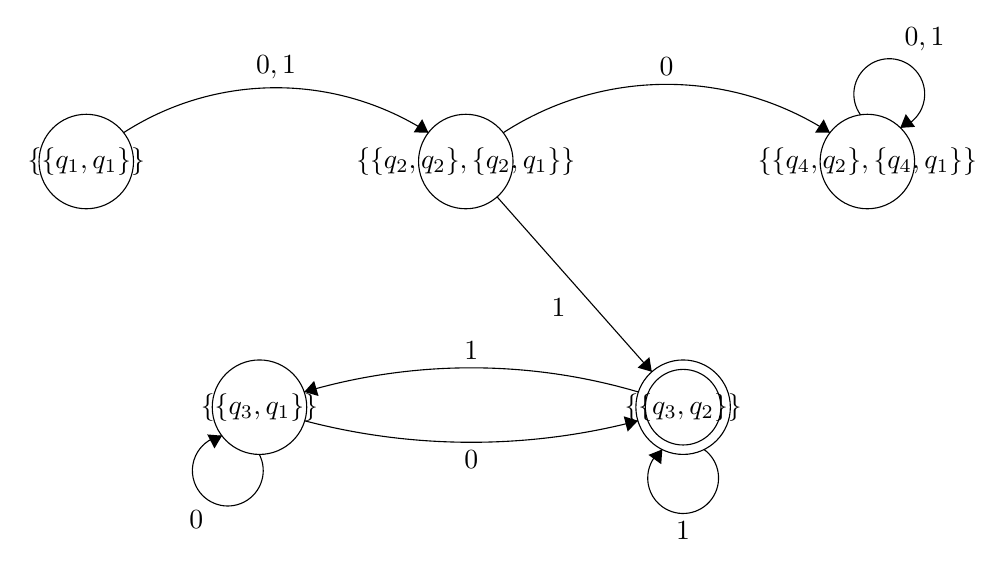
\begin{tikzpicture}[scale=0.2]
		\tikzstyle{every node}+=[inner sep=0pt]
		\draw [black] (12.5,-17.3) circle (3);
		\draw (12.5,-17.3) node {$\{\{q_1,q_1\}\}$};
		\draw [black] (36.6,-17.3) circle (3);
		\draw (36.6,-17.3) node {$\{\{q_2,q_2\},\{q_2,q_1\}\}$};
		\draw [black] (62.1,-17.3) circle (3);
		\draw (62.1,-17.3) node {$\{\{q_4,q_2\},\{q_4,q_1\}\}$};
		\draw [black] (23.5,-32.9) circle (3);
		\draw (23.5,-32.9) node {$\{\{q_3,q_1\}\}$};
		\draw [black] (50.4,-32.9) circle (3);
		\draw (50.4,-32.9) node {$\{\{q_3,q_2\}\}$};
		\draw [black] (50.4,-32.9) circle (2.4);
		\draw [black] (14.871,-15.468) arc (122.86351:57.13649:17.836);
		\fill [black] (34.23,-15.47) -- (33.83,-14.61) -- (33.29,-15.45);
		\draw (24.55,-12.11) node [above] {$0,1$};
		\draw [black] (38.976,-15.474) arc (123.02688:56.97312:19.033);
		\fill [black] (59.72,-15.47) -- (59.33,-14.62) -- (58.78,-15.46);
		\draw (49.35,-11.9) node [above] {$0$};
		\draw [black] (61.671,-14.343) arc (215.98629:-72.01371:2.25);
		\draw (65.73,-10.31) node [above] {$0,1$};
		\fill [black] (64.19,-15.16) -- (65.13,-15.1) -- (64.54,-14.29);
		\draw [black] (51.723,-35.58) arc (54:-234:2.25);
		\draw (50.4,-40.15) node [below] {$1$};
		\fill [black] (49.08,-35.58) -- (48.2,-35.93) -- (49.01,-36.52);
		\draw [black] (38.59,-19.55) -- (48.41,-30.65);
		\fill [black] (48.41,-30.65) -- (48.26,-29.72) -- (47.51,-30.39);
		\draw (42.96,-26.55) node [left] {$1$};
		\draw [black] (26.34,-31.935) arc (106.47249:73.52751:37.419);
		\fill [black] (26.34,-31.93) -- (27.25,-32.19) -- (26.97,-31.23);
		\draw (36.95,-29.9) node [above] {$1$};
		\draw [black] (47.528,-33.765) arc (-75.30417:-104.69583:41.697);
		\fill [black] (47.53,-33.76) -- (46.63,-33.48) -- (46.88,-34.45);
		\draw (36.95,-35.63) node [below] {$0$};
		\draw [black] (23.484,-35.888) arc (27.43495:-260.56505:2.25);
		\draw (19.49,-39.44) node [below] {$0$};
		\fill [black] (21.12,-34.71) -- (20.18,-34.63) -- (20.64,-35.52);
	\end{tikzpicture}
\end{center}

\end{minipage}
\newline
To prove minimality, we provide a distinguishing string $w$ for each pair of
states in the given DFA:
\begin{align*}
	\{\{q_1,q_1\}\}\text{ and }\{\{q_2,q_2\},\{q_2,q_1\}\}: 01\\
	\{\{q_1,q_1\}\}\text{ and }\{\{q_4,q_2\},\{q_4,q_1\}\}: 01\\
	\{\{q_1,q_1\}\}\text{ and }\{\{q_3,q_1\}\}: 001\\
	\{\{q_1,q_1\}\}\text{ and }\{\{q_3,q_2\}\}: 001\\
	\{\{q_2,q_2\},\{q_2,q_1\}\}\text{ and }\{\{q_4,q_2\},\{q_4,q_1\}\}: 1\\
	\{\{q_2,q_2\},\{q_2,q_1\}\}\text{ and }\{\{q_3,q_1\}\}: 01\\
	\{\{q_2,q_2\},\{q_2,q_1\}\}\text{ and }\{\{q_3,q_2\}\}: 01\\
	\{\{q_4,q_2\},\{q_4,q_1\}\}\text{ and }\{\{q_3,q_1\}\}: 1\\
	\{\{q_4,q_2\},\{q_4,q_1\}\}\text{ and }\{\{q_3,q_2\}\}: 1\\
	\{\{q_3,q_2\}\}\text{ and }\{\{q_3,q_1\}\}: 1\\
\end{align*}
We clearly see each pair of states is distinguishable, and so our DFA is minimal.
\section{} % Section 2
We construct an NFA recognizing One-off$(L)$ given the DFA recognizing
$L$, $M$.\\
We first define $M'$ to be the same as $M$, but with non-accepting states in
place of accepting states. Our NFA has a start state with $\varepsilon$-transitions
to $M'$'s start state, and to another state with a transition arrow for 0 and 1
going to the start state of $M$. We now create another accepting state with
transition arrows for 0 and 1 coming from every state in $M'$ that was an
accepting state in $M$.
\newline
\newline
We now have an NFA that accepts any string beginning with a 0 or a 1 followed by
a string in $L$, and also accepts any string beginning with a string in $L$
followed by a 0 or a 1. Thus, our NFA accepts One-off$(L)$.
\section{} % Section 3
\subsection{} % Section 3.a
We shall construct an NFA recognizing $A^R$ given the DFA recognizing $A$.
We first change all accepting states in the DFA to non-accepting states in the
NFA. Then, we reverse all transitions in the DFA, and create a new state with
$\varepsilon$-transtions to all former accepting states, and let it be the start
state. The former start state is now the single accepting state. We have now
constructed an NFA recognizing $A^R$, and so $A^R$ is regular.
\subsection{} % Section 3.b
\subsection*{i.} % Section 3.b.i
We showed above that $A^R$ is regular if $A$ is regular, and we know that the
regular languages are closed under concatenation. Thus, if $A$ and $B$ are
regular, then $A^RB^R=\{w^Ry^R|w\in A,y\in B\}$ is regular.
\subsection*{ii.} % Section 3.b.ii
We construct a DFA recognizing the language as follows:
\newline
\newline
Let $D_A=(Q_A,\Sigma_A,\delta_A,q_{0_A},F_A)$ and $D_B=(Q_B,\Sigma_B,\delta_B,q_{0_B},F_B)$
be DFAs recognizing $A$ and $B$, respectively.
\begin{align*}
	&Q=\{(q_i,q_j,x)|q_i\in A,q_j\in B,x\in\{0,1,2\ldots,2n\}\}\\
	&\Sigma=\Sigma_B\cup\Sigma_A\\
	&\delta((q_i,q_j,x),a)=\left\{
	\begin{array}{@{}ll@{}}
		(\delta_A(q_i,a),q_j,x+1)\text{ if $x\equiv0$ (mod 2)}\\
		(q_i,\delta_B(q_j,a),x+1)\text{ if $x\equiv1$ (mod 2)}
	\end{array}\right.\\
	&q_0=(q_{0_A},q_{0_B},0)\\
	&F=\{(q_i,q_j,2n)|q_i\in F_A,q_j\in F_B\}
\end{align*}
Our DFA follows both $D_A$ and $D_B$ in an alternating fashion and accepts only
when it has found an accepting string of length $n$ from both languages.
\section{} % Section 4
\subsection{} % Section 4.a
Only 2.
\subsection{} % Section 4.b
\begin{minipage}{\textwidth}
\begin{center}
	\begin{tikzpicture}[scale=0.2]
		\tikzstyle{every node}+=[inner sep=0pt]
		\draw [black] (21.7,-17.2) circle (3);
		\draw (21.7,-17.2) node {$q_1$};
		\draw [black] (51.6,-17.2) circle (3);
		\draw (51.6,-17.2) node {$q_2$};
		\draw [black] (51.6,-17.2) circle (2.4);
		\draw [black] (35.2,-33.3) circle (3);
		\draw (35.2,-33.3) node {$q_3$};
		\draw [black] (24.7,-17.2) -- (48.6,-17.2);
		\fill [black] (48.6,-17.2) -- (47.8,-16.7) -- (47.8,-17.7);
		\draw (36.65,-17.7) node [below] {$1$};
		\draw [black] (11.5,-17.2) -- (18.7,-17.2);
		\fill [black] (18.7,-17.2) -- (17.9,-16.7) -- (17.9,-17.7);
		\draw [black] (20.377,-14.52) arc (234:-54:2.25);
		\draw (21.7,-9.95) node [above] {$0$};
		\fill [black] (23.02,-14.52) -- (23.9,-14.17) -- (23.09,-13.58);
		\draw [black] (51.878,-14.225) arc (202.3925:-85.6075:2.25);
		\draw (56.14,-10.95) node [above] {$1$};
		\fill [black] (54.13,-15.61) -- (55.06,-15.77) -- (54.68,-14.84);
		\draw [black] (50.919,-20.119) arc (-17.62157:-73.43617:19.145);
		\fill [black] (38.13,-32.67) -- (39.04,-32.92) -- (38.75,-31.97);
		\draw (47.11,-28.46) node [below] {$0$};
		\draw [black] (36.275,-30.501) arc (155.47252:113.46975:24.451);
		\fill [black] (48.78,-18.22) -- (47.85,-18.08) -- (48.25,-19);
		\draw (39.62,-22.72) node [above] {$0,1$};
	\end{tikzpicture}
\end{center}

\end{minipage}
\begin{minipage}{\textwidth}
\begin{center}
	\begin{tikzpicture}[scale=0.2]
		\tikzstyle{every node}+=[inner sep=0pt]
		\draw [black] (30.1,-17.2) circle (3);
		\draw (30.1,-17.2) node {$q_1$};
		\draw [black] (48.8,-17.2) circle (3);
		\draw (48.8,-17.2) node {$q_2$};
		\draw [black] (36.9,-33.9) circle (3);
		\draw (36.9,-33.9) node {$q_3$};
		\draw [black] (16.5,-17.2) circle (3);
		\draw (16.5,-17.2) node {$q_0$};
		\draw [black] (64.6,-17.2) circle (3);
		\draw (64.6,-17.2) node {$q_4$};
		\draw [black] (64.6,-17.2) circle (2.4);
		\draw [black] (33.1,-17.2) -- (45.8,-17.2);
		\fill [black] (45.8,-17.2) -- (45,-16.7) -- (45,-17.7);
		\draw (39.45,-17.7) node [below] {$1$};
		\draw [black] (28.777,-14.52) arc (234:-54:2.25);
		\draw (30.1,-9.95) node [above] {$0$};
		\fill [black] (31.42,-14.52) -- (32.3,-14.17) -- (31.49,-13.58);
		\draw [black] (49.078,-14.225) arc (202.3925:-85.6075:2.25);
		\draw (53.34,-10.95) node [above] {$1$};
		\fill [black] (51.33,-15.61) -- (52.26,-15.77) -- (51.88,-14.84);
		\draw [black] (48.8,-20.195) arc (-5.48895:-65.45649:15.635);
		\fill [black] (39.73,-32.92) -- (40.67,-33.04) -- (40.25,-32.14);
		\draw (46.56,-29.15) node [right] {$0$};
		\draw [black] (37.346,-30.936) arc (167.08642:121.96815:19.759);
		\fill [black] (46.14,-18.59) -- (45.2,-18.59) -- (45.73,-19.44);
		\draw (39.92,-22.51) node [left] {$0,1$};
		\draw [black] (19.5,-17.2) -- (27.1,-17.2);
		\fill [black] (27.1,-17.2) -- (26.3,-16.7) -- (26.3,-17.7);
		\draw (23.3,-16.7) node [above] {$\epsilon$};
		\draw [black] (10.8,-17.2) -- (13.5,-17.2);
		\fill [black] (13.5,-17.2) -- (12.7,-16.7) -- (12.7,-17.7);
		\draw [black] (51.8,-17.2) -- (61.6,-17.2);
		\fill [black] (61.6,-17.2) -- (60.8,-16.7) -- (60.8,-17.7);
		\draw (56.7,-16.7) node [above] {$\epsilon$};
	\end{tikzpicture}
\end{center}

\end{minipage}
\begin{minipage}{\textwidth}
\begin{center}
	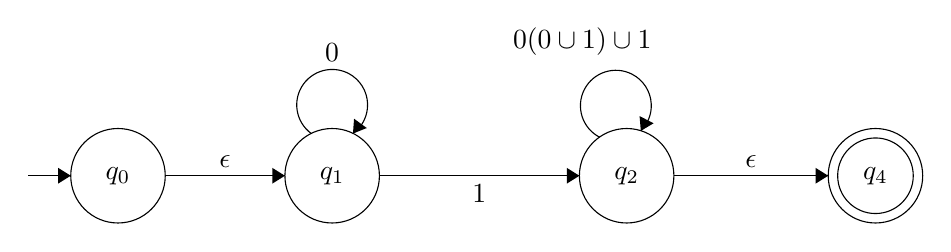
\begin{tikzpicture}[scale=0.2]
		\tikzstyle{every node}+=[inner sep=0pt]
		\draw [black] (30.1,-17.2) circle (3);
		\draw (30.1,-17.2) node {$q_1$};
		\draw [black] (48.8,-17.2) circle (3);
		\draw (48.8,-17.2) node {$q_2$};
		\draw [black] (16.5,-17.2) circle (3);
		\draw (16.5,-17.2) node {$q_0$};
		\draw [black] (64.6,-17.2) circle (3);
		\draw (64.6,-17.2) node {$q_4$};
		\draw [black] (64.6,-17.2) circle (2.4);
		\draw [black] (33.1,-17.2) -- (45.8,-17.2);
		\fill [black] (45.8,-17.2) -- (45,-16.7) -- (45,-17.7);
		\draw (39.45,-17.7) node [below] {$1$};
		\draw [black] (28.777,-14.52) arc (234:-54:2.25);
		\draw (30.1,-9.95) node [above] {$0$};
		\fill [black] (31.42,-14.52) -- (32.3,-14.17) -- (31.49,-13.58);
		\draw [black] (47.085,-14.753) arc (242.74686:-45.25314:2.25);
		\draw (45.98,-9.59) node [above] {$0(0\cup1)\cup1$};
		\fill [black] (49.7,-14.35) -- (50.51,-13.87) -- (49.62,-13.41);
		\draw [black] (19.5,-17.2) -- (27.1,-17.2);
		\fill [black] (27.1,-17.2) -- (26.3,-16.7) -- (26.3,-17.7);
		\draw (23.3,-16.7) node [above] {$\epsilon$};
		\draw [black] (10.8,-17.2) -- (13.5,-17.2);
		\fill [black] (13.5,-17.2) -- (12.7,-16.7) -- (12.7,-17.7);
		\draw [black] (51.8,-17.2) -- (61.6,-17.2);
		\fill [black] (61.6,-17.2) -- (60.8,-16.7) -- (60.8,-17.7);
		\draw (56.7,-16.7) node [above] {$\epsilon$};
	\end{tikzpicture}
\end{center}

\end{minipage}
\begin{minipage}{\textwidth}
\begin{center}
	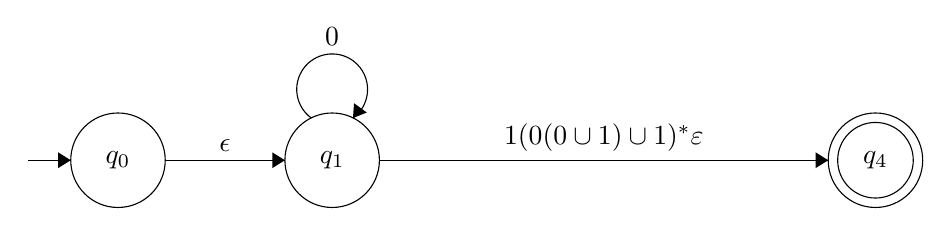
\begin{tikzpicture}[scale=0.2]
		\tikzstyle{every node}+=[inner sep=0pt]
		\draw [black] (30.1,-17.2) circle (3);
		\draw (30.1,-17.2) node {$q_1$};
		\draw [black] (16.5,-17.2) circle (3);
		\draw (16.5,-17.2) node {$q_0$};
		\draw [black] (64.6,-17.2) circle (3);
		\draw (64.6,-17.2) node {$q_4$};
		\draw [black] (64.6,-17.2) circle (2.4);
		\draw [black] (28.777,-14.52) arc (234:-54:2.25);
		\draw (30.1,-9.95) node [above] {$0$};
		\fill [black] (31.42,-14.52) -- (32.3,-14.17) -- (31.49,-13.58);
		\draw [black] (19.5,-17.2) -- (27.1,-17.2);
		\fill [black] (27.1,-17.2) -- (26.3,-16.7) -- (26.3,-17.7);
		\draw (23.3,-16.7) node [above] {$\epsilon$};
		\draw [black] (10.8,-17.2) -- (13.5,-17.2);
		\fill [black] (13.5,-17.2) -- (12.7,-16.7) -- (12.7,-17.7);
		\draw [black] (33.1,-17.2) -- (61.6,-17.2);
		\fill [black] (61.6,-17.2) -- (60.8,-16.7) -- (60.8,-17.7);
		\draw (47.35,-16.7) node [above] {$1(0(0\cup1)\cup1)^*\varepsilon$};
	\end{tikzpicture}
\end{center}

\end{minipage}
\begin{minipage}{\textwidth}
\begin{center}
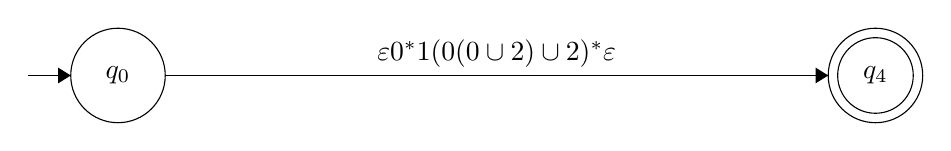
\begin{tikzpicture}[scale=0.2]
\tikzstyle{every node}+=[inner sep=0pt]
\draw [black] (16.5,-17.2) circle (3);
\draw (16.5,-17.2) node {$q_0$};
\draw [black] (64.6,-17.2) circle (3);
\draw (64.6,-17.2) node {$q_4$};
\draw [black] (64.6,-17.2) circle (2.4);
\draw [black] (10.8,-17.2) -- (13.5,-17.2);
\fill [black] (13.5,-17.2) -- (12.7,-16.7) -- (12.7,-17.7);
\draw [black] (19.5,-17.2) -- (61.6,-17.2);
\fill [black] (61.6,-17.2) -- (60.8,-16.7) -- (60.8,-17.7);
	\draw (40.55,-16.7) node [above] {$\varepsilon0^*1(0(0\cup2)\cup2)^*\varepsilon$};
\end{tikzpicture}
\end{center}

\end{minipage}
So the regular expression is $\varepsilon0^*1(0(0\cup2)\cup2)^*\varepsilon$.
\end{document}
